\documentclass[../main.tex]{subfiles}
\begin{document}


The setting of binary classification using the \zeroone-loss allows us to clearly distinguish two cases. An example may be classified correctly, in which case it does not contribute to the overall error. Otherwise, it is classified incorrectly and contributes exactly $1$.
While diversity-effect (in expectation over $(X,Y)$) is non-negative for ensembles of weak-learners (see theorem \ref{thm:todo}), there may still be example-outcome pairs that contribute negatively to the expectation, as illustrated in figures \ref{fig:zeroone-div-eff-good} and \ref{fig:zeroone-div-eff-bad}

\begin{marginfigure}
    \label{fig:zeroone-div-eff-good}
    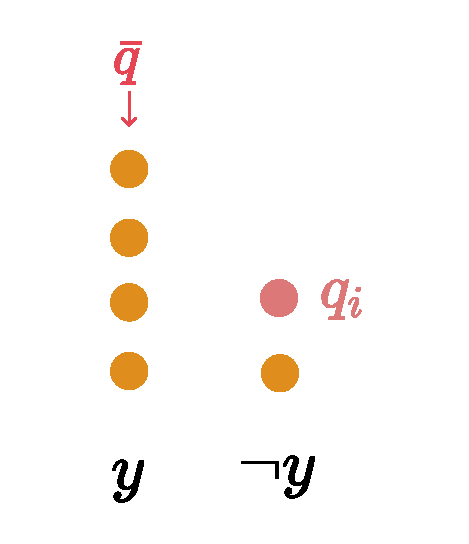
\includegraphics[width=0.8\textwidth]{figma-illustrations/zeroone-div-effect-good.pdf}
    \caption{
        Example of the effect of a member's vote $q_i$ on the diversity on a point for which the ensemble majority vote is correct.
    Example where $q_i$ has positive contribution to the diversity effect term, i.e. 
$\Lzo{y}{q_{i}} - \Lzo{y}{\bar{q}} = 1$. The member $q_{i}$ is incorrect but due to the discreteness of the majority vote combiner, the ensemble performance does not suffer -- unless the majority vote is tipped. Any correct vote while the ensemble already is correct is effectively "wasted" and incorrect votes correspond to diversity.
}
\end{marginfigure}
\begin{marginfigure}
    \label{fig:zeroone-div-eff-bad}
    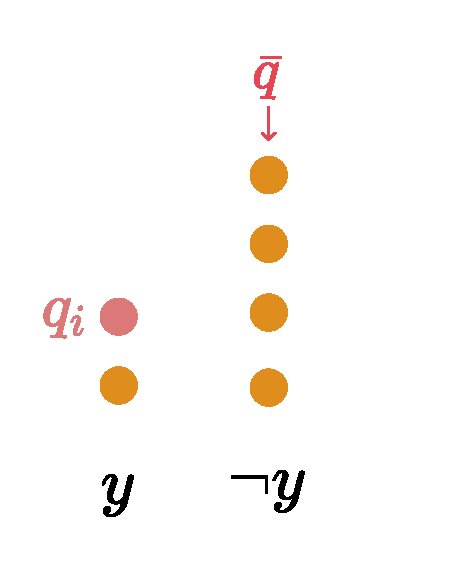
\includegraphics[width=0.8\textwidth]{figma-illustrations/zeroone-div-effect-bad.pdf}
    \caption{
    Example where $q_i$ has negative contribution to the diversity effect term, i.e. 
$\Lzo{y}{q_{i}} - \Lzo{y}{\bar{q}} = -1$. Any further incorrect vote while the ensemble is already incorrect would be wasted. The negative effect here eventually results in the \zeroone-loss of $1$.
}
\end{marginfigure}
\begin{lemma} (\cite{kuncheva})
For $y, \bar{q} \in \{ -1, 1 \}$ it holds that 
$$
\Mavg \left[\Lzo{y}{q_{i}} - \Lzo{y}{\bar{q}}\right] 
= (y \cdot \bar{q}) \Mavg \Lzo{\bar{q}}{q_{i}} \in \{-1, 0, 1\}
$$
\end{lemma}
\begin{proof} Let $y, \bar{q} \in \{ -1, 1 \}$.
\begin{itemize}
\item Assume the ensemble is correct, i.e. $y=\bar{q}$. Then $\Lzo{y}{\bar{q}} = 0$ and the left-hand-side equals $\Mavg\Lzo{y}{q_{i}} = \Mavg\Lzo{\bar{q}}{q_{i}}$. Further, $y \cdot \bar{q} = 1$.
\item Assume the ensemble is incorrect, i.e. $y \not= \bar{q}$. Then $y \cdot \bar{q} = -1$ and, for the left-hand-side, we can write
$$
\Mavg \left[\Lzo{y}{q_{i}}\right] - 1 = - \left(1 - \Mavg \Lzo{y}{q_{i}}\right) = - \left(\Mavg \Lzo{\bar{q}}{q_{i}} \right)
$$
using that, since $y \not= \bar{q}$, $\left(  1 - \Mavg \Lzo{y}{q_{i}}\right) = \Mavg \Lzo{\bar{q}}{q_{i}}$.
\end{itemize}
\end{proof}
% TODO rather, the below should be in a theorem box and the above should be the motivation/derivation/proof
This shows that, for binary classification under \zeroone-loss, diversity-effect can be decomposed exactly between points that contribute positively or negatively to the overall loss.
 Starting from the 
ambiguity-effect decomposition \ref{sec:ambiguity-effect-decomp}:
\marginnote{
An intuition of this is also that of "wasted votes": Under the majority vote combiner, for the ensemble to be correct, we require only at least half of the members to be correct. Any higher ratio of correct ensemble members does not improve the ensemble performance on this point and these can be seen as "wasted". Likewise, the ensemble is incorrect if not more than half of the members are correct. Any positive votes do not influence the ensemble improvement and can be considered "wasted". 
}

We can divide the range of $X$ into two disjoint subsets. Let $X_{+}$ be the examples on which the ensemble is correct. Ambiguity on these points has a decreasing effect on the overall ensemble error. Let $X_{-}$ be the examples on which the ensemble is incorrect. Ambiguity on these points has an increasing effect on the overall ensemble error. This yields a decomposition into \textit{good} and \textit{bad} diversity.

% TODO instead give this in terms ambiguity decomp here
\begin{widepar}
\begin{corollary} (\cite{kuncheva})
\begin{align*}
\mathbb{E}_{X}\left[   L(Y, \bar{q}) \right] 
&= 
\mathbb{E}_{X}\left[    \Mavg \Lzo{Y}{q_{i}}  \right]
-
\mathbb{E}_{X}\left[   \Mavg L(Y, q_{i}) - L(Y, \bar{q}) \right] \\
&= 
\mathbb{E}_{X}\left[ \Mavg \Lzo{Y}{q_{i}} \right] - \mathbb{E}_{X}\left[ (y \cdot \bar{q}) \Mavg \Lzo{\bar{q}}{q_{i}} \right]  \\
&= 
\mathbb{E}_{X}\left[    \Mavg \Lzo{Y}{q_{i}}  \right]
- 
\left(
\underbrace{
\mathbb{E}_{X_{+}}\left[ \Mavg \Lzo{\bar{q}}{q_{i}} \right]  
}_{\text{"good" diversity}}
- 
\underbrace{
\mathbb{E}_{X_{-}}\left[ \Mavg \Lzo{\bar{q}}{q_{i}} \right] 
}_{\text{"bad" diversity}}
\right)
\end{align*}
\end{corollary}
\end{widepar}
% TODO how does this relate to competence / weak learner assumption?

% TODO make indices, notation consistent and more comparable with other theorems
% TODO give a bit of reasoning why formally we can decompose expectation into X+, X-
% TODO key difference to covariance arguments is that members only need to be different to the combiner, and not necessarily disagree *with each other*?
% TODO marginfig with these functions
% TODO also intuition how other ensemble members "pulls" combiner into other direction
% TODO ok well obviously noted by kuncheva, but not exploited
\marginnote{
 Starting from the ambiguity decomposition:
$$
\Lzo{y}{\bar{q}} 
= \Mavg \Lzo{y}{q_{i}} - \left(\Mavg   \Lzo{y}{q_{i}} - \Lzo{y}{\bar{q}} \right)
$$
If $x \in X_{+}$, i.e. $\bar{q}(x) = y$:
$$
\Lzo{y}{\bar{q}} = 
\Mavg \Lzo{y}{q_{i}} - \left(\Mavg   \Lzo{y}{q_{i}} - 0 \right) = 0
$$
If $x \in X_{-}$, i.e. $\bar{q}(x) \not= y$:
$$
\Lzo{y}{\bar{q}} = 
\Mavg \Lzo{y}{q_{i}} - \left(\Mavg   \Lzo{y}{q_{i}} - 1 \right) = 1
$$       
}

As with any ambiguity decomposition, there is a tradeoff between average member error and diversity. Here, however, diversity is not always beneficial. On points where the ensemble is incorrect, disagreements have a negative effect on the overall ensemble error.
In other words, for majority vote ensembles, diversity is only beneficial \textit{on points at which the ensemble can actually afford to be diverse}. 

Further, from corollary \ref{above}, one can already see that the ensemble improvement (i.e. diversity-effect) is only non-negative if good diversity outweights bad diversity.

% As can be seen from the ambiguity decomposition of theorem \ref{thm:ambig-effect-decomp}, for diversity to be beneficial it has to mitigate the average member error. 
% % TODO clarify above sentence
% However, to the best of our knowledge, it has not yet been exploited that diversity is measured \textit{per point}.
% % TODO cite that paper in margin that does this via human-in-the-loop

Good and bad diversity can be expressed solely in terms of the number of incorrect members. 
\begin{lemma} $\star$ Let $y$ be the true outcome for a given example. Let $\neg y$ be an outcome that is not $y$. Write $\Lzo{q_i}{\neg y} \defeq \sum_{k \not= y} \Lzo{q_i}{k}$ for the indication whether $q_i$ is incorrect. Then the following identities hold.
% TODO y always first in losses
\begin{align*}
\mathbb{E}_{X_{+}}\left[ \Mavg \Lzo{q_{i}}{\bar{q}} \right] &=
\mathbb{E}_{X_{+}}\left[ \Wmem \right]   \\
\mathbb{E}_{X_{-}}\left[ \Mavg \Lzo{q_{i}}{\bar{q}} \right]  &= \mathbb{E}_{X_{-}}\left[ \Mavg  \Lzo{q_{i}}{\neg y} \right]  \\
&=
\mathbb{E}_{X_{-}}\left[ 1 - \Wmem \right]
\end{align*}
Analogous equalities hold in expectation over member parameter $\Theta$.
\end{lemma}

% TODO plots

% \sidenote{
%     This also gives a nice illustration of the Jury theorem (\ref{thm:jury}). If ensemble members are weak learners, i.e. they predict the correct class with probability greater than $\frac{1}{2}$, adding an additional learner is more likely to increase the good diversity term than the bad diversity term.
% % TODO check this
% }

% TODO I think we need to adjust this, get notation right for not \neg y in multiclass case

% TODO could sound reasonable to actively try not upweighting negative ones, or introduce sort of a slope in between


% TODO stress that weighting is *one* way to use this information, could also think about doing "dynamic" NCL

\subsection{Guiding ensemble construction with example weights}
\label{sec:guiding-ensemble-construction-with-example-weights}

(introduction ensemble construction, tree-by-tree with adaptive weights)

Now that we know exactly how correct and incorrect classifications affect the ensemble error, we will work towards leveraging this insight to find an ensemble construction scheme ...

% TODO what do we hope to gain? 
% - improved performance
% - same/similar performance but higher diversity -> lower variance (actually need to write part on ensemble variance reduction...)
% - same performance with fewer trees

% \marginfigfromsource{fig:weighting-fns}{symlinks/illustrations/weighting-fns/weighting-fns}
On points for which the ensemble is correct, diversity is beneficial and corresponds directly to the average member error. This means that we might expect to see an increase in ensemble performance if disagreement on correct points is encouraged -- as long as it does not cross the majority vote threshold. Indeed, in the perfect case, all examples would be correctly classified with a member error just below the majority vote threshold. This would result in an ensemble with large average member error but also with high diversity which mitigates the member error.

% TODO all the "sweet spot" ensemble guys saying that there's a region of equally good models do not even consider this

On points for whch the ensemble is incorrect, diversity hurts the ensemble performance. 
One could argue that, to minimise bad diversity, the average member error should be large, i.e. all members (instead of only some) should be driven to \textit{mis}-classify the example. However, we conjecture that this would cause the ensemble construction procedure to "give up" on misclassified examples. We will consider a different strategy first. Instead of giving up, the ensemble construction scheme should put more emphasis on these points, in the hope of eventually pushing it over the majority vote threshold towards a correct classification. This means that we are effectively \textit{increasing} bad diversity, in the hope that it eventually turns into good diversity.
% TODO plot of diversity-effect with the discont. around maj vote threshold

In standard Random Forests, each next tree is constructed independently of the ensemble constructed so far. Instead, we may try to construct the next tree in a coordinated manner such that it more optimally complements the ensemble constructed so far. 
Both good and bad diversity can be expressed in terms of the average member error. Each member that is added to the ensemble contributes to it. Consequently, we might be able to steer the development of ensemble performance by encouraging the next member to either correctly or inclassify a point, given how the ensemble constructed so far performs on this point.



We now proceed to define some weighting functions informed by diversity (see \ref{prev-section}).
% TODO plot it (only it) in margin
\marginnote{
   } 
\begin{definition} (DRF weighting scheme \cite{bernard-drf})
Let $\bar{q}$ be the ensemble constructed so far. For a pair $(X,Y) \in D$, define the \textit{Dynamic Random Forest weighting scheme} as 
$$
w_{\text{DRF}}(X) \defeq \Mavg \Lzo{Y}{q_{i}(X)}
$$
\label{def:drf-weighting-scheme}
\end{definition}
% TODO open over what $(X,Y)$ were really working here -- needs distinguishing also if we do weighted bootstrapping or weighted construction
This will have the effect that correctly classified examples are assigned lower weight and incorrectly classified examples are assigned higher weight.  % TODO will it really?

% TODO so, ensemble no longer homogeneous? like in boosting?

% TODO let's phrase this more like "turns out this already appears in literature, however with little to no theoretic motivation"
This weighting scheme was first proposed in \cite{bernard-drf}. However, they only give a heuristic, intuitive justification in that if a high number of trees misclassifies an example, the next tree should put more emphasis on it, similar to boosting strategies (\ref{sec:boosting}). We derive and motivate this weighting scheme from a perspective of diversity and give insight into how exactly it works -- namely, that it does \textit{not} flat-out increase the performance (as in boosting schemes) but instead encourages diversity.
% TODO not quite correct, more intricate

% TODO cite
XuChen re-iterate on the DRF weighting scheme and propose an alternative scheme.
$$
w_{\text{XuChen}}(X) \defeq \begin{cases}
\varepsilon^2 & \varepsilon \leq \frac{1}{2} \\ \\
\sqrt{\varepsilon} & \varepsilon > \frac{1}{2}
\end{cases}
\hspace{2em} \text{for~}  \varepsilon \defeq \Mavg \Lzo{Y}{q_i(X)}
$$
% TODO plot it in margin
Again, the authors provide only a heuristic motivation, which is that, compared to $w_{\text{DRF}}$, their method has a more drastic effect of up- and downweighting. We can now give a more informed interpretation. Inspecting $w_{\text{DRF}}$, which is continuous around the majority vote threshold, one can see that very similar weights are assigned to examples which are classified just barely correctly (resulting in a \zeroone-loss of $0$) and examples which are classified just barely incorrectly (resulting in a \zeroone-loss of $1$). This may mean suboptimal guidance in ensemble construction since both cases have very similar weights, but their effect on the ensemble loss is actually dramatically different. One disadvantage is that we take a heuristic step away from theory. % TODO wording


% TODO do try other weighting fns, maybe one that does not go all the way up on bad side but instead has sort of a bump in that it will attempt to move examples that are close to the threshold towards it but also to fully give up on examples that are close to full member error

% TODO relate this weighting to competence -- does it establish competence? can an ensemble be "more" competent? what interpretation does the competence inequality gap have?

Now we just have to figure out
% TODO wording
how to actually influence the training of the next member such that it's performance on some points is (likely) increased or decreased. One way that is suited well for Random Forests
% why exactly?
is to assign \textit{weights} $w: X \to [0,1]$ to examples and consider them during member training. 
In section \ref{sec:boosting-rationale-for-weights}, we will argue in detail how example weights influence the ensemble. % TODO

For random forests, these weights can possibly come into effect via two mechanisms:
% TODO main motivation for this weighting stuff was also that it is usable in RFs -- cannot just backprop or whatever
% -- although certanly thinkable, see negative correlation forests -- would actually expect to see a much stronger effect there
\begin{itemize}
    \item \textit{Weighted bootstrapping}: Instead of drawing the bootstrap samples uniformly, draw a sample with probability according to its weight. If the bootstrap sample is large, examples with higher weight are more likely to be oversampled and thus appear multiple times in the bootstrap sample. 
    \item \textit{Weighted tree construction}: We have seen in \ref{sec:decision trees} that tree construction according to some impurity measure greedily optimises a loss function. Likewise, weighting examples during computation of the impurity measure optimises a weighted loss.
\end{itemize}
% TODO dont need to consider leaf combiner because trees are deep

% TODO although somewhat similar in spirit, need to take care to distinguish this from boosting, because it really is something different altogether

\subsection{Experimental Evaluation of the DRF weighting schemes}

% TODO actually mention that it has already been shown that this approach is valid due to Bernard and XuChen -- recap results

% TODO overview: what are we trying to find out? Why are we comparing what we are comparing?
We compare different variants of the weighting scheme introduced in section \ref{sec:guiding-ensemble-construction-with-example-weights}. We look at the overall ensemble generalisation error, as well as the components of the error as given by the bias-variance decomposition \ref{todo} and the diversity decomposition \ref{todo}. Further, we analyse the ensemble margins (definition \ref{def:ensemble-margin}).

\subsubsection{Experiment Setup}
\label{sec:experiment-setup}



\paragraph{Compared learners} In summary, we compare the following learning algorithms. For a learner, any configuration is similar to the one mentioned before unless otherwise specified. Since for the weighted variants the construction of the next tree depends on the performance of the ensemble so far, trees are constructed in sequence.

% TODO somewhere. these hyperparams are not necessarily the best for the dataset, in particular the number of features.
\textit{standard-rf-classifier}: Standard Random Forest implementation based on \textit{sklearn}. The tree hyperparameters are such that trees are grown until each leaf contains one data point. The number of randomly sampled candidate dimensions to search for the best split is set to $\sqrt{d}$ where $d$ is the total number of dimensions. The impurity measure is the Gini impurity as defined in section \ref{sec:gini-impurity}. Each tree is grown on a bootstrap sample determined by sampling $n$ out of $n$ data points uniformly, with replacement.

\textit{drf-weighted-bootstrap-classifier}: Each tree is grown on a bootstrap sample determined by sampling $n$ out of $n$ points according to the DRF weighting scheme (see \ref{def:drf-weighting-scheme}). To yield a valid probability distribution, the weights are normalised via $w'(x_i) \gets \frac{w(x_i)}{\sum_{j=1}^n w(x_j)}$.

\textit{drf-weighted-fit-classifier}: Each tree is grown on a uniform bootstrap sample. For tree construction, namely measuring impurity, each example is weighted according to $w_{\text{DRF}}$ (again, normalised).

\textit{drf-weighted-fit-oob-classifier}: The example weights for a point $x_i$ are determined based only on \textit{out-of-bag} trees for $x_i$. These are those trees whose bootstrap sample has not included $x_i$.
% TODO don't forget to mention others here if we add some

\paragraph{Compared datasets} We give a brief motivation for the classification datasets we have selected for evaluation. A detailed summary of each dataset can be found in \ref{fig:grid}.
\cover is a dataset with a relatively high number of examples and low feature dimensionality. \mnist is a dataset with a moderate number of examples and high dimensionality. \diabetes is a dataset with relatively high error rates. \bioresponse is a small dataset with a very high number of features ($d \approx \frac{1}{2}n$). \qsar is a small dataset used for quick testing.
Further, \cite{bernard, xuChen} evaluated on \textit{mnist} (although not just a subset of it), \spambase, \digits and \diabetes.

\paragraph{Approximating statistical quantities} 
% how exactly are we approximating E_D and diversity stuff (3 trials)
For a dataset with $n$ examples, $n_{\text{train}} \defeq \frac{3}{4}n$ examples were assigned to be part of the \textit{training split}, the other $n_{\text{test}}$ for the \textit{testing split}. Examples in the testing split are used for evaluation only and were never used in training a model.
If $X$ is a random variable taking values in the space of examples $\mathcal{X}$, expectations over $X$ are approximated as the arithmetic mean over given examples in the testing split, i.e. for a function $g$:
$$
\mathbb{E}_X \left[ g(X) \right]  \approx \sum_{i=1}^{n_\text{test}} g(x_i)
$$
If $D$ is a random variable corresponding to the input to a learner, for instance the training dataset or randomness in the learning algorithm, an expectation over $D$ is approximated by an arithmetic mean over results of a fixed number of trials. In our case, we performed $3$ trials. % TODO maybe some sentence on how we didnt have capacity to optimise for performance that much, and couldnt wait that much for restuls.

\subsubsection{Results}

% TODO somewhere make it more clearly visible that we're actually getting improvement in generalisation error -- maybe even with table

We describe and analyse the results here and provide several plots. The full results plotted for comparison across learners and datasets are given in section \ref{sec:drf-full-results}.

\begin{figure*}
    \includegraphics{symlinks/zero-one-plots/bvd-decomps/spambase-openml/bvd.png}
    \caption{
        Comparison of components of the ensemble generalisation error on the \spambase dataset. Visualised are ensemble generalisation error, average member bias, average member variance and diversity.
        % TODO could actually exclude oob classifer .. never noteworthy over weighted-fit
    }
    \label{fig:spambase-bvd}
\end{figure*}



% would actually be interesting to BVD plots for each trial separately...

% always start to ask myself "okay, but are diverse models even better?"
% but I think that's not the right question to ask. diversity is a dimension of model fit, just like bias and variance. there'll always be interactions and tradeoffs. 


\paragraph{Generalisation error and diversity} 

\begin{marginfigure}
    \includegraphics[width=\textwidth]{symlinks/zero-one-plots/bvd-decomps/cover/get_diversity_effect.png}
    \caption{
        Diversity-effect by number of trees for different learners on the \cover dataset. Weighted bootstrapping amounts to a sharp increase in diversity for the first couple of trees. Weighted tree construction only causes a slight increase in diversity as compared to a standard Random Forest.
    }
    \label{fig:cover-diversity-effect}
\end{marginfigure}

\begin{marginfigure}
    \includegraphics[width=\textwidth]{symlinks/zero-one-plots/bvd-decomps/cover/get_expected_ensemble_loss.png}
    \caption{
        Expected generalisation error for different learners on the \cover dataset. Weighted tree construction and standard Random Forests behave almost identically. For weighted bootstrapping, an initial increase in error is followed by a consistently lower error rate.
%     % TODO fix colors of this -- probably best if they're all gray but have different line styles 
    }
    \label{fig:cover-ensemble-loss}
\end{marginfigure}

% \begin{marginfigure}
%     \includegraphics[width=\textwidth]{symlinks/zero-one-plots/bvd-decomps/mnist_subset/get_expected_ensemble_loss.png}
%     \caption{
%     }
%     % TODO fix colors of this -- probably best if they're all gray but have different line styles 
%     \label{fig:mnist-ensemble-loss}
% \end{marginfigure}

% \begin{marginfigure}
%     \includegraphics[width=\textwidth]{symlinks/zero-one-plots/bvd-decomps/mnist_subset/bvd-individual/drf-weighted-bootstrap-classifier.png}
%     \caption{
%         TODO
%     }
%     \label{fig:mnist-bvd}
% \end{marginfigure}


% putting this here for the time being for better layout...
\begin{marginfigure}
    \includegraphics[width=\textwidth]{symlinks/zero-one-plots/bvd-decomps/digits/bvd-individual/drf-weighted-bootstrap-classifier.png}
    \caption{
        Ensemble generalisation error, ensemble bias and ensemble variance of weighted bootstrapping on the \digits dataset. 
    }
    \label{fig:digits-bvd}
\end{marginfigure}


% \begin{marginfigure}
%     \includegraphics[width=\textwidth]{symlinks/zero-one-plots/bvd-decomps/digits/bvd-individual/drf-weighted-bootstrap-classifier.png}
%     \caption{
%         Ensemble generalisation error, ensemble bias and ensemble variance of weighted bootstrapping on the \digits dataset. 
%     }
%     \label{fig:digits-ens}
% \end{marginfigure}

% TODO reference diversity tradeoff

%
We can see that weighted bootstrapping and weighted tree construction (see \ref{sec:guiding-ensemble-constr}) behave quite differently. The case for the \spambase dataset is given in \reffig{fig:cover-bvd}. 

It is striking that, for every dataset, weighted bootstrapping initially brings a sharp increase in average bias and, consequently, generalisation error. The average variance stays mostly constant after an initial slight increase. As the number of trees grows, the generalisation error and the average bias diminish. A sharp initial increase in diversity mitigates the increase in average bias. The average bias then continously decreases to a similar or slightly higher level as the other learners. The average member variance seems to be very similar to that of other learners.

Weighted bootstrapping seems to be able to achieve similar or, often, better generalisation error than any other learner.  It also consistently produces higher diversity ensembles than the other learners.
It is interesting to note that on \spambase, where the initial increase in average bias and diversity appear most pronounced, diversity actually \textit{decreases} as more trees are added to the ensemble. 
% TODO can we give an explanation / interpretation why that would be?

For weighted tree construction, average bias and average variance are mostly constant and the decrease in generalisation error with a growing number of trees is solely due to increasing diversity. This is the same behaviour we also observe and motivate theoretically for standard Random Forests. Weighted tree construction performans as good as or slightly worse than standard Random Forests in terms of generalisation error. This is somewhat surprising since the intuitive motivation was that weighted tree construction will influence the splitting criteria. 

Weighted tree contruction with out-of-bag weights does not appear to bring any advantage.


% \begin{figure*}
%     \includegraphics{symlinks/zero-one-plots/bvd-decomps/cover/bvd.png}
%     \caption{
%         todo
%     }
%     \label{fig:cover-bvd}
% \end{figure*}

% \begin{figure*}
%     \includegraphics{symlinks/zero-one-plots/bvd-decomps/bioresponse/bvd.png}
%     \caption{
%         Example of a dataset for which weighting does not give an advantage. \bioresponse is an extremely high-dimensional dataset where the number of features is more than half the number of training datapoints.
%         Visualised are ensemble generalisation error, average member bias, average member variance and diversity.
%         % TODO could actually exclude oob classifer .. never noteworthy over weighted-fit
%     }
%     \label{fig:cover-bvd}
% \end{figure*}

\paragraph{Ensemble bias and variance} 
%
The initial increase in average bias is also reflected in an initial increase in ensemble bias. At the same time, ensemble variance is decreased. 
Note how the average variance stays almost constant, while the ensemble variance varies greatly. 
This is the "outside view" on how diversity is a component of ensemble variance.


As the number of trees grows, for some datasets, ensemble variance is higher. For others, it is similar to standard Random Forests.

% \begin{figure*}
%     \includegraphics{symlinks/zero-one-plots/bvd-decomps/mnist_subset/ens.png}
%     \caption{
%         todo
%     }
%     \label{fig:mnist-en}
% \end{figure*}

\paragraph{Ensemble margins} 
\begin{figure*}
    \includegraphics{symlinks/zero-one-plots/margins/spambase-openml/margins.png}
    \caption{
        Ratio of incorrect trees per number of trees in the ensemble, plotted separately for correctly (green) and incorrectly (red) classified examples. 
    }
    \label{fig:mnist-en}
\end{figure*}
\begin{marginfigure}
    \includegraphics[width=\textwidth]{symlinks/zero-one-plots/margins/diabetes/standard-rf-classifier/by-example-50.png}
    \includegraphics[width=\textwidth]{symlinks/zero-one-plots/margins/diabetes/drf-weighted-bootstrap-classifier/by-example-50.png}
    \caption{
        Histograms of ensemble margins per example for the standard Random Forest (top) and weighted bootstrapping (bottom) learners grown each of $M=50$ trees on the \diabetes dataset. For weighted bootstrapping, the distribution of the margins appears slightly skewed to the center, reflecting that the weighting schemes encourages disagreement on points where many ensemble members are correct and agreement on points where many ensemble members are incorrect.
    }
    \label{fig:cover-margins-50}
\end{marginfigure}
The weighting schemes are essentially thought of to influence the ratio of incorrect members and thus bias, variance and diversity. Under the weighting schemes defined in \ref{todo}, on points for which the ensemble prediction is correct, the ratio of incorrect trees should \textit{increase} (more diversity) and on points for which the ensemble prediction is incorrect, the ratio of incorrect trees should \textit{decrease}.
We can directly observe the ratio of incorrect members. We plot the average ratio of incorrect trees $\Mavg \Lzo(y, q_i)$ separately for correctly and incorrectly classified examples. For weighted bootstrapping, across all datasets, we can indeed observe the expected effect. This is another view on the sharply increasing diversity as seen in e.g. figure \ref{fig:spambase-bvd}. Again, the effect diminishes as the number of trees grows.

% TODO add margins plotting to DVC pipeline!
% TODO in plots, use same order of datasets/learners as in other grids
Further, we can look at the distribution of ensemble margin per example. We plot a histogram of examples with respect to the number of trees incorrectly classifying that example. In binary classification, more than $\frac{1}{2}M$ trees being incorrect leads to an incorrect ensemble prediction. % TODO what about multi-class?
For instance for the \cover dataset, we can observe that the distribution of ensemble margins indeed seems to be skewed slightly to the right (i.e. in direction of more disagreement) for positive examples (see \reffig{fig:cover-margins-50})

% also: oob estimation more computationally expensive? certainly harder to implement. also don't really see the motivation too much.

% Full results are given in detail and for comparison with each other in \ref{sec:drf-full-results}.

% brown2005 p1639 hints at that flexible diversity learning may be linked to noisy data

\paragraph{Comparing weighted bootstrapping and weighted tree construction} It is worth discussing why weighted bootstrapping and weighted tree construction produce such different behaviour. 
%
% Under weighted bootstrapping, examples are sampled according to a non-uniform probability distribution determined by the weights. This means that, in expectation, each example appears with a frequency according to its weight in the bootstrap sample.
% %
% With uniform bootstrapping and weighted tree construction, since each example is sampled according to the same probability, in expectation, each example appears with the same frequency in a bootstrap sample. However, in tree construction, the examples are then weighted. 
%
% It seems intuitive that both approaches should yield very similar results. However, one key difference can be identified. 
In practise, any bootstrap sample is finite. The bootstrap sample is drawn with replacement, thus a bootstrap sample does not necessarily include all examples from the training dataset. 
%
Under uniform bootstrapping, each example has equal chance to be included in the bootstrap sample (see \ref{sec:bagging}). It is then considered during tree construction according to its weight. On the other hand, under weighted bootstrapping, examples with high weight are more likely and examples with low weight are less likely to appear in the bootstrap sample. In particular, this means that examples with low weight are more likely to not be included at all in the bootstrap sample and consequently not be considered at all during tree construction. 
%
This might be an intuitive explanation why weighted bootstrapping shows a stronger effect than weighted tree construction in our experiments.  A thorough discussion has to be left for future work. 



\paragraph{Comparison to \cite{bernard-drf}} 

\citeauthor{bernard-drf} evaluated only the following approach: They would perform both weighted bootstrapping and weighted tree construction. Further, weights would be determined only on out-of-bag-trees (see section \ref{sec:experiment-setup}). Additionally, unrelated to the question at hand, they also employed a different way to determine candidate split features. Unlike in standard random forests, where a fixed number of candidate split features is sampled from all available features, the number of sampled candidate features was left fully random here. It was left unanswered which of these components actually affect the ensemble to what extent. Further, they did not provide any explanation or empirical analysis in terms of diversity.
Looking at our results, the following points seem likely:
\begin{itemize}
    \item An improvement in generalisation error is still obtained with standard candidate split feature sampling.
    \item The improvement can be explained using the notions of diversity.
    \item Weighted tree construction alone appears to have only very little effect as compared to a standard Random Forest.
    \item Weighted bootstrapping seems to provide the main effect.
    \item Determination of weights using out-of-bag-trees only does not improve performance for weighted tree construction. 
    % TODO adress overfitting thoguths from DRF paper
    % my intuition is that overfitting is not an issue here
\end{itemize}

% TODO bernard states that fewer trees are needed -- can we, too, observer this?

% Xu_Chen report the following
% TABLE II. AVERAGE ERROR RATES (IN \%) OF THE RF MADE OF 500 TREES, FOR THE 3 RF INDUCTION ALGORITHMS. 
% uses oob estimation, doesnt seem to use improved feature selection
% \begin{array}{|c|c|c|c|}
% \hline \text { Datasets } & \text { RF } & \text { DRF } & \text { Optimized DRF } \\
% \hline \text { Diabetes } & 23.6 & 23.58 & \mathbf{2 3 . 4 2} \\
% \hline
% \end{array}

% bernard report
% \begin{array}{|l|c|c|c|}
% \hline \text { Datasets } & \text { BRF } & \text { F-RK } & \text { DRF } \\
% \hline \hline \text { Diabetes } & 25.25 & 24.86 & \mathbf{2 4 . 5 9} \\
% \hline \text { Digits } & 2.28 & 2.21 & \mathbf{2 . 1 0} \\
% \hline
% \end{array}
% \begin{array}{|l|c|c|c|}
% \hline \text { Datasets } & \text { BRF } & \text { F-RK } & \text { DRF } \\
% \hline \text { MNIST } & 4.97 & 4.95 & \mathbf{4 . 6 1} \\
% \hline \text { Spambase } & 4.88 & 5.03 & \mathbf{4 . 0 4} \\
% \hline
% \end{array}



\paragraph{Ambiguity-effect decomp plots} ...
% TODO actually understand what is going on here.

\paragaraph{Scatter Plots} ...
% TODO where each member is a point and axes are diversity (ie. LE to centroid) and member error
% -- like in Zhou2012 p. 110, because people did that with other measures

\end{document}